\documentclass[tikz]{standalone}
\usetikzlibrary{positioning}

\newcommand{\po}[2]{\draw [->, thick] (#1) to node[above] {\Large{so}} (#2);}
\newcommand{\povis}[2]{\draw [->, thick] (#1) to node[above] {\Large{\texttt{so}}$,$\Large{\texttt{vis}}$,$\Large{\texttt{ar}}} (#2);}
%p\newcommand{\povis}[2]{\draw [->, thick] (#1) to node[above] {\Large{so}} node[below] {\Large{vis}} (#2);}
\newcommand{\vis}[2]{\draw [->, thick] (#1) to node[above, sloped] {$\Large{\texttt{vis},\texttt{ar}}$} (#2);}
\newcommand{\ar}[2]{\draw [->, thick, dotted] (#1) to node[above, sloped] {\Large{\texttt{ar}}} (#2);}
\newcommand{\vvis}[2]{\draw [->, thick, dashed, allow upside down] (#1) to node[above, sloped] {\Large{\texttt{vis}}$,$\Large{\texttt{ar}}} (#2);}

\renewcommand{\wr}{\texttt{wr}}
\newcommand{\rd}{\texttt{rd}}

\begin{document}
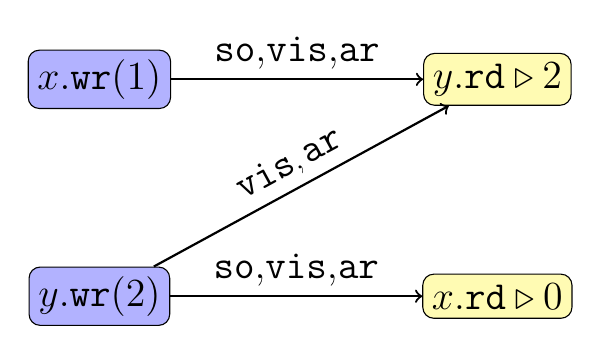
\begin{tikzpicture}
\tikzset{
  wop/.style = {rectangle, rounded corners, fill = blue!30, draw, font = \Large},
  rop/.style = {rectangle, rounded corners, fill = yellow!30, draw, font = \Large}, process/.style = {font = \huge},
  %po/.style = {->, very thick},
  rw/.style = {->, shorten >= 3pt, very thick, dashed},
  %vis/.style = {->, shorten >= 3pt, very thick, dashed}
}

  \node (wx1) [wop] {$x.\wr(1)$};
  \node (ry2) [rop, right = 3.2cm of wx1] {$y.\rd\triangleright 2$};

  \node (wy2) [wop, below = 2 of wx1] {$y.\wr(2)$};
  \node (rx0) [rop, right = 3.2cm of wy2] {$x.\rd\triangleright 0$};

  \povis{wx1}{ry2};
  \povis{wy2}{rx0};

  \vis{wy2}{ry2};

\end{tikzpicture}
\end{document}
